\lecture{7}{Designing Powerful Graph Encoders: Breaking the Limits of the WL Kernel}{Tuesday, October 13, 2026}\label{ch:lec07}

% Notation used in this lecture (bold, as in macros.tex)
\providecommand{\vc}{\mathbf{c}}
\providecommand{\mC}{\mathbf{C}}
\providecommand{\mV}{\mathbf{V}}
\providecommand{\mLambda}{\bm{\Lambda}}

% Local TikZ styles (prefix lec07)
\tikzset{
  lec07v/.style={circle, draw=black!75, fill=white, semithick, minimum size=4.6mm,
                 inner sep=0pt, font=\scriptsize},
  lec07d/.style={circle, fill=black!65, minimum size=1.7mm, inner sep=0pt},
  lec07e/.style={black!70, semithick},
  lec07lbl/.style={font=\scriptsize\sffamily},
  lec07A/.style={font=\scriptsize\sffamily, text=BurntOrange},
  lec07B/.style={font=\scriptsize\sffamily, text=TealBlue},
  lec07w0/.style={circle, draw=black!60, fill=white, minimum size=3.9mm,
                  inner sep=0pt, font=\tiny\itshape},
  lec07w1/.style={lec07w0, draw=blue!45, fill=blue!25},
  lec07w2/.style={lec07w0, draw=blue!80!black, fill=blue!75!black, text=white},
}

\textbf{Outline.} Limitations of GNNs (a ``perfect'' GNN; structure- vs.\
position-aware failures) $\to$ a spectral perspective of message-passing GNNs
(GIN in matrix form, eigendecomposition of $\mA$, spectral limitation of the WL
kernel) $\to$ feature augmentation: eigenvector-based GNNs (Laplacian
eigenvectors) $\to$ feature augmentation: structurally-aware GNNs (cycle counts,
closed loops) $\to$ position-aware GNNs (anchors, anchor-sets, P-GNN).

% ---------------------------------------------------------------------
\section{Limitations of graph neural networks}\label{sec:lec07-limits}

\subsection{Recap and a ``perfect'' GNN}\label{sec:lec07-perfect}
\slides{3--6}

\begin{itemize}
  \item \textbf{Recap -- GNN training pipeline} (\cref{ch:lec05}): input graph
    $\to$ GNN $\to$ node embeddings $\to$ prediction head $\to$ predictions;
    + labels $\to$ loss function, evaluation metrics; dataset split.
    \textbf{Today's lecture: can we make GNN representation more expressive?}
  \item \textbf{A thought experiment: what should a perfect GNN do?}
    \begin{itemize}
      \item A $k$-layer GNN embeds a node based on the $K$-hop neighborhood
        structure (figure: $k=1$, $k=2$ rings; aggregator$_1$, aggregator$_2$).
      \item A perfect GNN should build \textbf{an injective function} between
        \textbf{neighborhood structure (regardless of hops)} and \textbf{node
        embeddings}.
    \end{itemize}
  \item \textbf{For a perfect GNN} (ignore node attributes for now; attributes of
    all nodes are the same):
    \begin{itemize}
      \item \term{Observation 1}: if two nodes have \textbf{the same} neighborhood
        structure, they \textbf{must have the same embedding} (ex.\ $v_1$, $v_2$
        each in a triangle: $h_{v_1}=h_{v_2}$).
      \item \term{Observation 2}: if two nodes have \textbf{different}
        neighborhood structure, they \textbf{must have different embeddings}
        (ex.\ $v_1$ in a triangle, $v_3$ in a square: $h_{v_1}\neq h_{v_3}$).
    \end{itemize}
\end{itemize}

\subsection{Imperfections of existing GNNs; plan}\label{sec:lec07-imperfect}
\slides{7--9}

\begin{itemize}
  \item \textbf{Observation 2 often cannot be satisfied} [You et al.,
    \emph{Identity-aware GNNs}, AAAI 2021]:
    \begin{itemize}
      \item The GNNs we have introduced so far are not perfect; their expressive
        power is \textbf{upper bounded by the WL test} (\cref{ch:lec06}).
      \item E.g.\ message passing GNNs \textbf{cannot count the cycle length}:
        $v_1$ in a cycle of length 3, $v_2$ in a cycle of length 4 $\Rightarrow$
        the computational graphs for $v_1$ and $v_2$ are always the same binary
        tree (ignoring node attributes) (as in \cref{ch:lec05}).
    \end{itemize}
  \item \textbf{Observation 1 could also have issues} [You, Ying, Leskovec,
    \emph{Position-aware GNNs}, ICML 2019]:
    \begin{itemize}
      \item Even though two nodes may have the same neighborhood structure, we may
        want to assign different embeddings to them, because they appear in
        \textbf{different positions in the graph}. We call these tasks
        \term{position-aware tasks}.
      \item \textbf{Even a perfect GNN will fail for these tasks:} e.g.\ a grid
        graph ($v_1$, $v_2$ at opposite corners); NYC road network ($v_1$, $v_2$
        two street locations).
    \end{itemize}
  \item \textbf{Plan:} resolve both issues by \textbf{building more expressive
    GNNs}.
    \begin{itemize}
      \item \textbf{Fix Observation 2:} build message passing GNNs that are more
        expressive than the WL test; example method: \textbf{structurally-aware
        GNNs} (\cref{sec:lec07-struct}).
      \item \textbf{Fix Observation 1:} create node embeddings based on their
        positions in the graph; example method: \textbf{position-aware GNNs}
        (\cref{sec:lec07-pos}).
    \end{itemize}
\end{itemize}

% ---------------------------------------------------------------------
\section{A spectral perspective of message-passing GNNs}\label{sec:lec07-spectral}

\subsection{More failure cases; limitation of the WL kernel}\label{sec:lec07-failures}
\slides{11--15}

\begin{itemize}
  \item GNNs exhibit \textbf{three levels of failure cases in structure-aware
    tasks} (node, edge, graph level) [You et al.\ AAAI 2021]. Each time:
    \textbf{different inputs but the same computational graph $\to$ GNN fails}.
    \begin{itemize}
      \item \textbf{Node level:} $v_1$ (label A) in a triangle vs.\ $v_2$ (label
        B) in a square $\Rightarrow$ same binary-tree computational graphs
        (as in \cref{ch:lec06}).
      \item \textbf{Edge level:} edges A $=(v_0,v_1)$ and B $=(v_0,v_2)$ share
        node $v_0$; we look at embeddings for $v_1$ and $v_2$ $\Rightarrow$ same
        computational graphs (\cref{fig:lec07-fail}a).
      \item \textbf{Graph level:} graphs A and B; we look at embeddings for each
        node $\Rightarrow$ for each node, the computational graph is the same in A
        and B (\cref{fig:lec07-fail}b).
    \end{itemize}
  \item \textbf{Limitation of the WL kernel} (graphs $\mathcal{G}$, $\hat{\mathcal{G}}$
    of \cref{fig:lec07-wlsym}, same WL colors):
    \begin{itemize}
      \item The WL kernel colors \textbf{inherit the graph symmetries}.
      \item \textbf{Symmetric colors} are associated with limitations involving the
        \textbf{spectral decomposition of the graph}.
    \end{itemize}
\end{itemize}

\begin{figure}[htbp]
  \centering
  \begin{subfigure}[b]{0.44\textwidth}
    \centering
    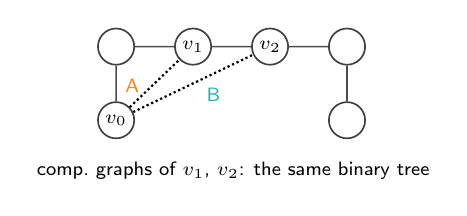
\begin{tikzpicture}[scale=0.85]
      \node[lec07v] (x)  at (0,1.1) {};
      \node[lec07v] (v1) at (1.15,1.1) {$v_1$};
      \node[lec07v] (v2) at (2.3,1.1) {$v_2$};
      \node[lec07v] (y)  at (3.45,1.1) {};
      \node[lec07v] (v0) at (0,0) {$v_0$};
      \node[lec07v] (z)  at (3.45,0) {};
      \draw[lec07e] (x)--(v1)--(v2)--(y) (x)--(v0) (y)--(z);
      \draw[densely dotted, thick] (v0)--(v1) node[lec07A, pos=0.45, left=1pt] {A};
      \draw[densely dotted, thick] (v0)--(v2) node[lec07B, pos=0.55, below right=-1pt] {B};
      \node[lec07lbl, align=center] at (1.75,-0.75)
        {comp.\ graphs of $v_1$, $v_2$: the same binary tree};
    \end{tikzpicture}
    \caption{Edge level (slide~13).}
  \end{subfigure}\hfill
  \begin{subfigure}[b]{0.52\textwidth}
    \centering
    \begin{tikzpicture}[scale=0.85]
      \foreach \i in {0,...,7} {
        \node[lec07d] (a\i) at ({90-45*\i}:0.85) {};
        \node[lec07d] (b\i) at ($(3.2,0)+({90-45*\i}:0.85)$) {};}
      \foreach \i in {0,...,7} {
        \pgfmathtruncatemacro{\j}{mod(\i+1,8)}
        \pgfmathtruncatemacro{\k}{mod(\i+2,8)}
        \pgfmathtruncatemacro{\m}{mod(\i+3,8)}
        \draw[lec07e] (a\i)--(a\j) (a\i)--(a\k) (b\i)--(b\j) (b\i)--(b\m);}
      \node[lec07A] at (0.95,0.95) {A};
      \node[lec07B] at (2.25,0.95) {B};
      \node[lec07lbl] at (1.6,-1.25) {each node: the same computational graph};
    \end{tikzpicture}
    \caption{Graph level: 8-cycle + chords to 2nd (A) / 3rd (B) neighbors
    (slide~14).}
  \end{subfigure}
  \caption{More GNN failure cases: different inputs, same computational graph
  (slides~13--14).}
  \label{fig:lec07-fail}
\end{figure}

\subsection{Matrix representation of GIN}\label{sec:lec07-matrix}
\slides{16--30}

\begin{itemize}
  \item \textbf{Recall the GIN update} (GINConv of \cref{ch:lec06}, now with layer
    $l$ and color vectors $\vc_v^{(l)}$):
\end{itemize}
\begin{equation}\label{eq:lec07-gin}
  \vc_v^{(l+1)} = \mathrm{MLP}\Big((1+\epsilon)\,\vc_v^{(l)}
    + \sum_{u\in\mathcal{N}(v)}\vc_u^{(l)}\Big)
\end{equation}
\begin{itemize}
  \item \textbf{We can consider a single-layer MLP} ($\sigma$ is a pointwise
    activation):
\end{itemize}
\begin{align}
  \vc_v^{(l+1)} &= \sigma\Big(\mW^{(l)}(1+\epsilon)\,\vc_v^{(l)}
    + \mW^{(l)}\sum_{u\in\mathcal{N}(v)}\vc_u^{(l)}\Big)\label{eq:lec07-gin1}\\
  \vc_v^{(l+1)} &= \sigma\Big(\mW_0^{(l)}\vc_v^{(l)}
    + \mW_1^{(l)}\sum_{u\in\mathcal{N}(v)}\vc_u^{(l)}\Big)\label{eq:lec07-gin2}
\end{align}
\begin{itemize}
  \item \Cref{eq:lec07-gin2} = \textbf{GraphSAGE with sum aggregation!} Computed as a
    \textbf{sparse matrix-vector multiplication} (see linear algebra recitation).
  \item \textbf{Neighborhood aggregation as matrix-vector mult.\ Key object:
    adjacency matrix $\mA$.} Example: path $v_1$--$v_2$--$v_3$--$v_4$; stack the
    colors as rows of $\mC^{(l)}$:
\end{itemize}
\begin{equation}\label{eq:lec07-Apath}
  \mA=\begin{pmatrix}0&1&0&0\\1&0&1&0\\0&1&0&1\\0&0&1&0\end{pmatrix},
  \qquad
  \mC^{(l)}\in\R^{N\times d},\quad \mC^{(l)}[v,:]=\vc_v^{(l)}
\end{equation}
\begin{itemize}
  \item The neighbor sum $\sum_{u\in\mathcal{N}(v)}\vc_u^{(l)}$ is row $v$ of
    $\mA\mC^{(l)}$ (the 1s of row $v$ of $\mA$ pick the neighbors' rows of
    $\mC^{(l)}$; slide~22 draws $\mC^{(l)}$ with rows
    $\vc^{(l)}_{v_1},\dots,\vc^{(l)}_{v_4}$):
\end{itemize}
\begin{equation}\label{eq:lec07-ACrows}
  \begin{aligned}
    \mA\mC^{(l)}[1,:]&=\vc_{v_2}^{(l)}, &\qquad
    \mA\mC^{(l)}[2,:]&=\vc_{v_1}^{(l)}+\vc_{v_3}^{(l)},\\
    \mA\mC^{(l)}[3,:]&=\vc_{v_2}^{(l)}+\vc_{v_4}^{(l)}, &\qquad
    \mA\mC^{(l)}[4,:]&=\vc_{v_3}^{(l)}
  \end{aligned}
\end{equation}
\begin{itemize}
  \item \textbf{Color update in matrix form}, where $\mA\in\{0,1\}^{N\times N}$ is
    the adjacency matrix: $\mA[u,v]=1$ if $(u,v)$ is an edge, $\mA[u,v]=0$ if
    $(u,v)$ is not an edge:
\end{itemize}
\begin{equation}\label{eq:lec07-ginmat}
  \mC^{(l+1)} = \sigma\Big(\mC^{(l)}\mW_0^{(l)} + \mA\mC^{(l)}\mW_1^{(l)}\Big)
  = \sigma\Big(\sum_{k=0}^{1}\mA^k\mC^{(l)}\mW_k^{(l)}\Big)
\end{equation}

\subsection{Spectral graph representation; GNNs as functions of eigenvectors}\label{sec:lec07-eig}
\slides{31--35}

\begin{itemize}
  \item \textbf{Eigenvalue decomposition of the graph adjacency matrix $\mA$:}
\end{itemize}
\begin{equation}\label{eq:lec07-eig}
  \mA = \mV\mLambda\mV^T
\end{equation}
\begin{itemize}
  \item $\mV=[\vv_1,\dots,\vv_n]$ is the orthonormal matrix of eigenvectors;
    $\mLambda$ is the diagonal matrix of eigenvalues $\{\lambda_n\}_{n=1}^N$.
    \begin{itemize}
      \item The eigenvalue (\textbf{spectral}) decomposition of the adjacency is a
        \textbf{universal characterization} of the graph.
      \item \textbf{Non-isomorphic graphs have different spectral
        decompositions.}
      \item The \textbf{number of cycles} in a graph can be viewed as
        \textbf{functions of eigenvalues and eigenvectors}, e.g.
    \end{itemize}
\end{itemize}
\begin{equation}\label{eq:lec07-tri}
  \#\text{triangles} = \diag\big(\mA^3\big) = \sum_{n=1}^{N}\lambda_n^3\,\abs{\vv_n}^2
\end{equation}
\begin{caution}
  Slides~31, 38 say ``$\#$triangles $=\diag(\mA^3)$''; correct: $\diag(\mA^3)_i$
  (closed 3-walks at node $i$, $\abs{\vv_n}^2$ element-wise) $=2\times$ the
  triangles through node $i$.
\end{caution}
\begin{itemize}
  \item \textbf{We can interpret GIN layers as MLPs operating on the
    eigenvectors:} replace $\mA$ in \cref{eq:lec07-ginmat} with the spectral
    decomposition $\mA=\mV\mLambda\mV^T$:
\end{itemize}
\begin{equation}\label{eq:lec07-ginspec}
  \mC^{(l+1)} = \sigma\Big(\sum_{k=0}^{1}\mA^k\mC^{(l)}\mW_k^{(l)}\Big)
  = \sigma\Big(\sum_{k=0}^{1}\mV\mLambda^k\,\mV^T\mC^{(l)}\,\mW_k^{(l)}\Big)
\end{equation}
\begin{itemize}
  \item The GNN update depends on the \textbf{eigenvalues, eigenvectors} and the
    \textbf{dot product} between the \textbf{eigenvectors} and the \textbf{colors
    at the previous level} ($\mV^T\mC^{(l)}$).
  \item \textbf{Recall color refinement} (slide~34 repeats the two-graph example
    of \cref{ch:lec06}): every node starts with color 1 $\Rightarrow$ uniform
    initial colors.
  \item \textbf{GNN with uniform initial colors:} $\mC^{(0)}=\vone$, so
\end{itemize}
\begin{equation}\label{eq:lec07-uniform}
  \mV^T\mC^{(0)} = \mV^T\vone,\qquad
  \mV^T\vone = \big[\langle\vv_1,\vone\rangle,\dots,\langle\vv_n,\vone\rangle\big]
\end{equation}
\begin{itemize}
  \item The new node colors \textbf{depend} on the \textbf{eigenvectors that are
    not orthogonal to $\vone$}.
  \item \textbf{Graphs with symmetries} admit \textbf{eigenvectors orthogonal to
    $\vone$}.
\end{itemize}

\subsection{Spectral limitation of the WL kernel}\label{sec:lec07-wllimit}
\slides{36--39}

\begin{itemize}
  \item \textbf{The WL kernel cannot distinguish between some basic graph
    structures}, e.g.\ $\mathcal{G}$ (two hexagons sharing edge $E$--$F$) vs.\
    $\hat{\mathcal{G}}$ (two pentagons joined by edge $E$--$F$)
    (\cref{fig:lec07-wlsym}). Their eigenvalues differ (\cref{tab:lec07-spec}).
  \item With $\langle\vv_n,\vone\rangle$ added (slide~37): the eigenpairs with
    $\langle\vv_n,\vone\rangle\neq0$ are the same in both graphs
    ($2.303/3.048$, $1/{-0.816}$, $-1.303/{-0.210}$); differing eigenvalues, e.g.\
    the boxed $\hat\lambda=1.861$, have $\langle\hat\vv_n,\vone\rangle=0$.
  \item \textbf{The WL kernel cannot count basic graph structures} (slide~38):
    $\#$triangles is a function of $\lambda_n$ and $\vv_n$ (\cref{eq:lec07-tri}),
    same table.
\end{itemize}

\begin{figure}[htbp]
  \centering
  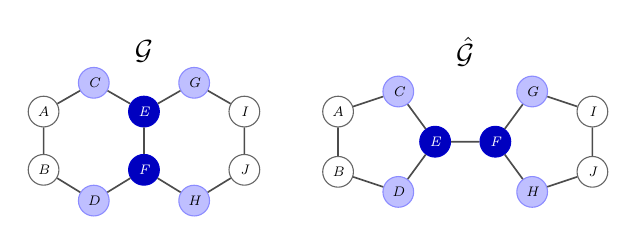
\begin{tikzpicture}[scale=0.85]
    % graph G: two hexagons sharing edge E--F
    \foreach \n/\s/\x/\y in {A/0/0/0.45, B/0/0/-0.42, C/1/0.75/0.88, D/1/0.75/-0.88,
        E/2/1.5/0.45, F/2/1.5/-0.42, G/1/2.25/0.88, H/1/2.25/-0.88,
        I/0/3.0/0.45, J/0/3.0/-0.42}
      \node[lec07w\s] (g\n) at (\x,\y) {\n};
    \draw[lec07e] (gA)--(gC)--(gE)--(gF)--(gD)--(gB)--(gA)
      (gE)--(gG)--(gI)--(gJ)--(gH)--(gF);
    \node at (1.5,1.35) {$\mathcal{G}$};
    % graph G-hat: two pentagons joined by edge E--F
    \begin{scope}[shift={(4.4,0)}]
      \foreach \n/\s/\x/\y in {A/0/0/0.45, B/0/0/-0.45, C/1/0.9/0.75, D/1/0.9/-0.75,
          E/2/1.45/0, F/2/2.35/0, G/1/2.9/0.75, H/1/2.9/-0.75,
          I/0/3.8/0.45, J/0/3.8/-0.45}
        \node[lec07w\s] (h\n) at (\x,\y) {\n};
      \draw[lec07e] (hA)--(hC)--(hE)--(hD)--(hB)--(hA) (hE)--(hF)
        (hF)--(hG)--(hI)--(hJ)--(hH)--(hF);
      \node at (1.9,1.35) {$\hat{\mathcal{G}}$};
    \end{scope}
  \end{tikzpicture}
  \caption{$\mathcal{G}$ vs.\ $\hat{\mathcal{G}}$: the WL colors (dark: $E,F$;
  light: $C,D,G,H$; white: $A,B,I,J$) are the same in both graphs and inherit
  their symmetries (slides~15, 36--38).}
  \label{fig:lec07-wlsym}
\end{figure}

\begin{table}[htbp]
  \centering\footnotesize
  \caption{Adjacency eigenvalues and $\langle\vv_n,\vone\rangle$ of $\mathcal{G}$
  and $\hat{\mathcal{G}}$; boxed column on slides~37--38 in bold (slides~36--38).}
  \label{tab:lec07-spec}
  \setlength{\tabcolsep}{3.6pt}
  \begin{tabular}{@{}ll|rrrrrrrrrr@{}}
    \toprule
    $\mathcal{G}$ & $\lambda_n$ & 2.303 & 1.618 & 1.303 & 1 & 0.618 & $-2.303$
      & $-1.618$ & $-0.618$ & $-1$ & $-1.303$\\
    & $\langle\vv_n,\vone\rangle$ & 3.048 & 0 & 0 & $-0.816$ & 0 & 0 & 0 & 0 & 0
      & $-0.210$\\
    \midrule
    $\hat{\mathcal{G}}$ & $\hat\lambda_n$ & 2.303 & \textbf{1.861} & 1 & 0.618
      & 0.618 & 0.254 & $-1.303$ & $-1.618$ & $-1.618$ & $-2.115$\\
    & $\langle\hat\vv_n,\vone\rangle$ & 3.048 & \textbf{0} & $-0.816$ & 0 & 0 & 0
      & $-0.210$ & 0 & 0 & 0\\
    \bottomrule
  \end{tabular}
\end{table}

\begin{keyidea}[Limitations of the WL kernel (slide 39)]
  \textbf{The limitations of the WL kernel are limitations of the initial node
  color.}
  \begin{itemize}
    \item These limitations are well understood in the \textbf{spectral domain}:
      constant node colorings are orthogonal with adjacency eigenvectors and
      \textbf{critical spectral components} (eigenvalues and eigenvectors)
      \textbf{are omitted}.
    \item At a high level, colors generated by the WL kernel obey the \textbf{same
      symmetries as graph structure}.
    \item These joint symmetries \textbf{lock} the message-passing operations to
      limited representations.
  \end{itemize}
\end{keyidea}

% ---------------------------------------------------------------------
\section{Feature augmentation: eigenvector-based GNNs}\label{sec:lec07-eigfeat}
\slides{41--44}

\begin{itemize}
  \item \textbf{What if we use eigenvectors as additional features?}
  \item \textbf{Key object:} \term{Laplacian matrix} $\mL$ = Degrees $-$
    Adjacency. Each graph has its own Laplacian matrix; the Laplacian encodes the
    graph structure; several Laplacian variants add degree information
    differently. Path $v_1$--$v_2$--$v_3$--$v_4$:
\end{itemize}
\begin{equation}\label{eq:lec07-lap}
  \mL = \mD - \mA
  = \underbrace{\begin{pmatrix}1&0&0&0\\0&2&0&0\\0&0&2&0\\0&0&0&1\end{pmatrix}}_{\text{degree of each node}}
  - \underbrace{\begin{pmatrix}0&1&0&0\\1&0&1&0\\0&1&0&1\\0&0&1&0\end{pmatrix}}_{\text{adjacency}}
\end{equation}
\begin{itemize}
  \item Laplacian matrix captures graph structure; \textbf{its eigenvectors
    inherit this structure}.
  \item \textbf{Eigenvectors with small eigenvalue = global structure, large
    eigenvalue = local symmetries.} (Figure from Kreuzer*, Beaini* et al.\ 2021:
    one eigenvector $\phi$ drawn on a graph of linked rings; $\lambda_1=0.037$
    varies smoothly from $-$max on one side to max on the other; $\lambda_2=0.1$;
    $\lambda_{10}=\lambda_{11}=1.0$ are nonzero only on a few rings.)
  \item \textbf{Refresher:} eigenvector $\vv$ such that ($\mL$: $n\times n$
    matrix; $\vv$: $n$-dimensional vector; $\lambda$: scalar eigenvalue)
    \begin{equation}\label{eq:lec07-eigvec}
      \mL\vv=\lambda\vv
    \end{equation}
  \item \textbf{Laplacian eigenvector positional encodings -- feature augmentation
    steps:} (1) compute $k$ eigenvectors (e.g.\ $\vv_1,\vv_2,\vv_3$, $k=3$); (2)
    stack into an $n\times k$ matrix ($n$ nodes); (3) the $i$th row is a feature
    for node $i$.
  \item \textbf{Laplacian eigenvectors in practice.} Task: given a graph, predict
    YES if it has a cycle, NO otherwise. ``PE'' = feature augmentation with
    Laplacian eigenvector (\cref{tab:lec07-pe}): PE helps at every training size;
    GatedGCN without PE stays at $50.000$.
\end{itemize}

\begin{table}[htbp]
  \centering\footnotesize
  \caption{Cycle detection: test accuracy $\pm$ s.d.\ vs.\ number of training
  samples (slide~44).}
  \label{tab:lec07-pe}
  \setlength{\tabcolsep}{4pt}
  \begin{tabular}{@{}lcc|cccc@{}}
    \toprule
    & & & \multicolumn{4}{c}{Train samples}\\
    Model & $L$ & \#Param & 200 & 500 & 1000 & 5000\\
    \midrule
    GIN & 4 & 100774 & 70.585$\pm$0.636 & 74.995$\pm$1.226 & 78.083$\pm$1.083
      & 86.130$\pm$1.140\\
    GIN-PE & 4 & 102864 & \textbf{86.720$\pm$3.376} & \textbf{95.960$\pm$0.393}
      & \textbf{97.998$\pm$0.300} & \textbf{99.570$\pm$0.089}\\
    \midrule
    GatedGCN & 4 & 103933 & 50.000$\pm$0.000 & 50.000$\pm$0.000 & 50.000$\pm$0.000
      & 50.000$\pm$0.000\\
    GatedGCN-PE & 4 & 105263 & \textbf{95.082$\pm$0.346} & \textbf{96.700$\pm$0.381}
      & \textbf{98.230$\pm$0.473} & \textbf{99.725$\pm$0.027}\\
    \bottomrule
  \end{tabular}
\end{table}

% ---------------------------------------------------------------------
\section{Feature augmentation: structurally-aware GNNs}\label{sec:lec07-struct}

\subsection{Our approach; the naive solution}\label{sec:lec07-naive}
\slides{46--49}

\begin{itemize}
  \item \textbf{We use the following thinking:}
    \begin{itemize}
      \item Two different inputs (nodes, edges, graphs) are labeled differently.
      \item A ``failed'' model will always assign \textbf{the same embedding} to
        them; a ``successful'' model will assign \textbf{different embeddings}.
      \item \textbf{Embeddings are determined by GNN computational graphs.} Ex.:
        two inputs $v_1$ (triangle) and $v_2$ (square), different labels A and B;
        goal: assign different embeddings to $v_1$ and $v_2$.
    \end{itemize}
  \item \textbf{A naive solution: one-hot encoding.} Encode each node with a
    different ID, then we can always differentiate different nodes/edges/graphs.
    \begin{itemize}
      \item Ex.: triangle: $v_1=1000$, others $0100$, $0001$; square: $v_2=1000$,
        others $0100$, $0001$, $0010$ $\Rightarrow$ $v_1$'s children $0100,0001$
        vs.\ $v_2$'s $0010,0100$: computational graphs are clearly different if
        each node has a different ID.
      \item \textbf{Issues:} \textbf{not scalable} -- need $\bigO(N)$ feature
        dimensions ($N$ is the number of nodes); \textbf{not inductive} -- cannot
        generalize to new nodes/graphs.
    \end{itemize}
  \item Constant vs.\ one-hot feature augmentation (slide~49) repeats the table
    of \cref{ch:lec05} (abbreviated in \cref{tab:lec07-structfeat}).
\end{itemize}

\subsection{Cycle counts and closed loops}\label{sec:lec07-cycles}
\slides{50--53}

\begin{itemize}
  \item \textbf{(2) Certain structures are hard to learn by GNN} -- solution:
    cycle count as augmented node features, starting from length 0 (slide~50
    repeats \cref{ch:lec05}: triangle $[0,0,0,1,0,0]$, square
    $[0,0,0,0,1,0]$).
  \item \term{ID-GNN-Fast} [You et al.\ AAAI 2021]: \textbf{ID-GNN rooted
    subtrees} mark the nodes that are the root itself (identity) $\Rightarrow$
    $v_1$ (A) $\neq$ $v_2$ (B). \textbf{Cycle count at each level:} $v_1$:
    $[1,0,2,2]$, $v_2$: $[1,0,2,0]$ (length-3 cycles $=2$ vs.\ $0$).
    \begin{itemize}
      \item \textbf{Idea:} count cycles originating from a given node, use it as
        initial feature.
      \item Include identity information as an \textbf{augmented node feature};
        \textbf{use cycle counts in each layer as an augmented node feature}. Also
        can be used together with \textbf{any GNN}.
    \end{itemize}
  \item \term{Closed loops as node features} [Kanatsoulis \& Ribeiro, \emph{Graph
    Neural Networks Are More Powerful Than We Think}, ICASSP 2024]: use the
    \textbf{diagonals of the adjacency powers} as augmented node features; they
    correspond to the \textbf{closed loops} each node is involved in:
\end{itemize}
\begin{equation}\label{eq:lec07-loops}
  \mC^{(0)} = \Big[\diag\big(\mA^0\big), \diag\big(\mA^1\big), \diag\big(\mA^2\big),
    \diag\big(\mA^3\big), \dots, \diag\big(\mA^{D-1}\big)\Big]
  \in \N_0^{N\times D}
\end{equation}
\begin{itemize}
  \item Augmented node feature for $v_1$: in a cycle with length 3:
    $[1,0,2,2,6,8]$; length 4: $[1,0,2,0,8,0]$.
\end{itemize}
\begin{caution}
  Slide~52: triangle feature $[1,0,2,2,6,8]$; correct: $[1,0,2,2,6,10]$
  ($\diag(\mA^5)=10$ for a triangle).
\end{caution}
\begin{proposition}[Expressive power; Kanatsoulis \& Ribeiro, ICASSP 2024]\label{prop:lec07-loops}
  If two graphs have adjacency matrices with \textbf{different eigenvalues}, there
  exists a GNN with closed-loop initial node features that can \textbf{always tell
  them apart}.
\end{proposition}
\begin{itemize}
  \item GNNs with \textbf{structural initial node features} can produce different
    representations for \textbf{almost all real-world graphs}.
  \item GIN with structural initial node features is \textbf{strictly more
    powerful} than the WL kernel.
\end{itemize}

\subsection{Other structural features}\label{sec:lec07-otherfeat}
\slides{54--55}

\begin{itemize}
  \item Other commonly used augmented features: \textbf{clustering coefficient},
    \textbf{PageRank}, \textbf{centrality}, \dots{} Any feature we have
    introduced in Lecture 1 can be used!
  \item \textbf{Constant vs.\ structure-aware} node features:
    \cref{tab:lec07-structfeat}.
\end{itemize}

\begin{table}[htbp]
  \centering\small
  \caption{Feature augmentation: constant vs.\ one-hot (slide~49, abbreviated
  from \cref{ch:lec05}) vs.\ structure-aware (slide~55).}
  \label{tab:lec07-structfeat}
  \renewcommand{\arraystretch}{1.15}
  \begin{tabularx}{\textwidth}{@{}>{\raggedright\arraybackslash}p{2.3cm}
      >{\raggedright\arraybackslash}p{2.2cm}>{\raggedright\arraybackslash}p{2.2cm}
      >{\raggedright\arraybackslash}X@{}}
    \toprule
    & Constant & One-hot & Structure-aware node feature\\
    \midrule
    Expressive power & Medium & High & \textbf{High.} Each node has a
      structure-aware ID, so node-specific information can be stored\\
    Inductive learning & High & Low & \textbf{High.} Simple to generalize to new
      nodes: can count triangles or closed loops for any graph\\
    Computational cost & Low & High & \textbf{Low/High.} Depending on the
      structures we are counting\\
    Use cases & Any graph, inductive & Small graph, transductive & Any graph,
      inductive settings (generalize new nodes)\\
    \bottomrule
  \end{tabularx}
\end{table}

% ---------------------------------------------------------------------
\section{Position-aware graph neural networks}\label{sec:lec07-pos}

\subsection{Structure-aware vs.\ position-aware tasks}\label{sec:lec07-tasks}
\slides{57--59}

\begin{itemize}
  \item \textbf{Two types of tasks on graphs} [You, Ying, Leskovec, ICML 2019]
    (\cref{fig:lec07-pos}a,b):
    \begin{itemize}
      \item \term{Structure-aware task}: nodes are labeled by their
        \textbf{structural roles} in the graph.
      \item \term{Position-aware task}: nodes are labeled by their
        \textbf{positions} in the graph.
    \end{itemize}
  \item \textbf{Structure-aware tasks: GNNs work} (we showed how to design GNNs
    to work well for them) -- can differentiate $v_1$ and
    $v_2$ by using different computational graphs ($v_1$: 2 neighbors; $v_2$: 3
    neighbors).
  \item \textbf{Position-aware tasks: GNNs will always fail} -- $v_1$ and $v_2$
    will always have the same computational graph, \textbf{due to structure
    symmetry}. \textbf{Can we define deep learning methods that are
    position-aware?}
\end{itemize}

\subsection{Anchors and anchor-sets}\label{sec:lec07-anchors}
\slides{60--62}

\begin{itemize}
  \item \textbf{Power of ``anchor'':} randomly pick a node $s_1$ as an \term{anchor
    node}; represent $v_1$ and $v_2$ via their relative distances w.r.t.\ $s_1$,
    \textbf{which are different} ($v_1$: 1, $v_2$: 2). An anchor node serves as
    \textbf{a coordinate axis}, which can be used to \textbf{locate nodes in the
    graph}.
  \item \textbf{Power of ``anchors'':} pick more nodes $s_1,s_2$ as anchor nodes
    (relative distances $v_1$: $(1,2)$, $v_2$: $(2,1)$). \textbf{Observation:} more
    anchors can better characterize node position in different regions of the
    graph; many anchors $\to$ many coordinate axes.
  \item \textbf{Power of ``anchor-sets'':} generalize anchor from a single node to
    \textbf{a set of nodes}; distance to an \term{anchor-set} = the minimum distance
    to all the nodes in the anchor-set.
    \begin{itemize}
      \item \textbf{Observation:} large anchor-sets can sometimes provide more
        precise position estimate $\Rightarrow$ we can save the total number of
        anchors.
      \item Ex.\ (\cref{fig:lec07-pos}c): size-2 anchor-set $s_3=\{v_3, s_1\}$;
        anchors $s_1,s_2$ cannot differentiate nodes $v_1,v_3$, but anchor-set
        $s_3$ can.
    \end{itemize}
\end{itemize}

\begin{figure}[htbp]
  \centering
  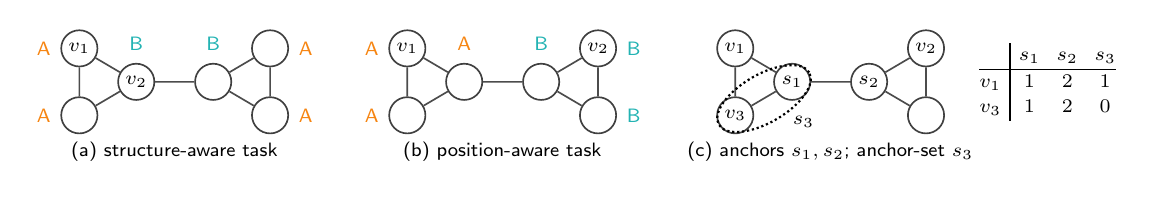
\begin{tikzpicture}[scale=0.85]
    % (a) structure-aware task
    \node[lec07v] (a1) at (0,0.5) {$v_1$};  \node[lec07v] (a2) at (0,-0.5) {};
    \node[lec07v] (a3) at (0.85,0) {$v_2$}; \node[lec07v] (a4) at (2.0,0) {};
    \node[lec07v] (a5) at (2.85,0.5) {};    \node[lec07v] (a6) at (2.85,-0.5) {};
    \draw[lec07e] (a1)--(a2)--(a3)--(a1) (a3)--(a4) (a4)--(a5)--(a6)--(a4);
    \node[lec07A, left] at (a1.west) {A}; \node[lec07A, left] at (a2.west) {A};
    \node[lec07B, above=1pt] at (a3.north) {B}; \node[lec07B, above=1pt] at (a4.north) {B};
    \node[lec07A, right] at (a5.east) {A}; \node[lec07A, right] at (a6.east) {A};
    \node[lec07lbl] at (1.42,-1.05) {(a) structure-aware task};
    % (b) position-aware task
    \begin{scope}[shift={(4.9,0)}]
      \node[lec07v] (b1) at (0,0.5) {$v_1$};  \node[lec07v] (b2) at (0,-0.5) {};
      \node[lec07v] (b3) at (0.85,0) {};      \node[lec07v] (b4) at (2.0,0) {};
      \node[lec07v] (b5) at (2.85,0.5) {$v_2$}; \node[lec07v] (b6) at (2.85,-0.5) {};
      \draw[lec07e] (b1)--(b2)--(b3)--(b1) (b3)--(b4) (b4)--(b5)--(b6)--(b4);
      \node[lec07A, left] at (b1.west) {A}; \node[lec07A, left] at (b2.west) {A};
      \node[lec07A, above=1pt] at (b3.north) {A}; \node[lec07B, above=1pt] at (b4.north) {B};
      \node[lec07B, right] at (b5.east) {B}; \node[lec07B, right] at (b6.east) {B};
      \node[lec07lbl] at (1.42,-1.05) {(b) position-aware task};
    \end{scope}
    % (c) anchors and anchor-set
    \begin{scope}[shift={(9.8,0)}]
      \node[lec07v] (c1) at (0,0.5) {$v_1$};    \node[lec07v] (c2) at (0,-0.5) {$v_3$};
      \node[lec07v] (c3) at (0.85,0) {$s_1$};   \node[lec07v] (c4) at (2.0,0) {$s_2$};
      \node[lec07v] (c5) at (2.85,0.5) {$v_2$}; \node[lec07v] (c6) at (2.85,-0.5) {};
      \draw[lec07e] (c1)--(c2)--(c3)--(c1) (c3)--(c4) (c4)--(c5)--(c6)--(c4);
      \draw[densely dotted, thick, rotate around={30:(0.43,-0.25)}]
        (0.43,-0.25) ellipse (0.78 and 0.36);
      \node[font=\scriptsize] at (1.02,-0.6) {$s_3$};
      \node[lec07lbl, align=center] at (1.42,-1.05) {(c) anchors $s_1,s_2$;
        anchor-set $s_3$};
    \end{scope}
    \node[font=\scriptsize, anchor=west] at (13.3,0) {%
      \setlength{\tabcolsep}{3pt}%
      \begin{tabular}{@{}c|ccc@{}}
        & $s_1$ & $s_2$ & $s_3$\\ \hline
        $v_1$ & 1 & 2 & 1\\
        $v_3$ & 1 & 2 & 0
      \end{tabular}};
  \end{tikzpicture}
  \caption{Two triangles joined by an edge: (a) structure-aware and (b)
  position-aware labels; (c) anchors and a size-2 anchor-set with the relative
  distances (= position encodings) of $v_1$, $v_3$ (slides~57--62, 66).}
  \label{fig:lec07-pos}
\end{figure}

\subsection{Anchor-set theory: Bourgain theorem and P-GNN}\label{sec:lec07-bourgain}
\slides{63--65}

\begin{itemize}
  \item \textbf{Goal:} embed the metric space $(V,d)$ into the Euclidean space
    $\R^k$ such that the original distance metric is preserved: for every node
    pair $u,v\in V$, the Euclidean embedding distance $\norm{\vz_u-\vz_v}_2$ is
    close to the original distance metric $d(u,v)$.
\end{itemize}
\begin{proposition}[Bourgain Theorem, informal; Bourgain 1985]\label{prop:lec07-bourgain}
  Consider the following embedding function of node $v\in V$:
  \begin{equation}\label{eq:lec07-bourgain}
    f(v) = \Big(d_{\min}(v,S_{1,1}), d_{\min}(v,S_{1,2}), \dots,
      d_{\min}(v,S_{\log n,\,c\log n})\Big) \in \R^{c\log^2 n}
  \end{equation}
  where $c$ is a constant; $S_{i,j}\subset V$ is chosen by including each node in
  $V$ independently with probability $\frac{1}{2^i}$; and
  \begin{equation}\label{eq:lec07-dmin}
    d_{\min}(v,S_{i,j}) \equiv \min_{u\in S_{i,j}} d(v,u).
  \end{equation}
  \textbf{The embedding distance produced by $f$ is provably close to the original
  distance metric $(V,d)$.}
\end{proposition}
\begin{itemize}
  \item \term{P-GNN} \textbf{follows the theory of Bourgain theorem:} first samples
    $\bigO(\log^2 n)$ anchor sets $S_{i,j}$; embeds each node $v$ via
    \cref{eq:lec07-bourgain}.
  \item \textbf{P-GNN maintains the inductive capability:} during training, new
    anchor sets are \emph{re-sampled} every time; P-GNN is learned to operate over
    the new anchor sets; at test time, given a new unseen graph, new anchor sets
    are sampled.
\end{itemize}

\subsection{Position encoding and how to use it}\label{sec:lec07-pe}
\slides{66--68}

\begin{itemize}
  \item \term{Position encoding for graphs}: represent a node's position by its
    distance to randomly selected anchor-sets; \textbf{each dimension} of the
    position encoding is \textbf{tied to an anchor-set} (\cref{fig:lec07-pos}c:
    $v_1$'s position encoding $(1,2,1)$, $v_3$'s $(1,2,0)$).
  \item \textbf{The simple way:} use position encoding as an augmented node feature
    (works well in practice).
    \begin{itemize}
      \item \textbf{Issue:} since each dimension of position encoding is tied to a
        random anchor set, dimensions of positional encoding can be randomly
        permuted, without changing its meaning.
      \item Imagine you permute the input dimensions of a normal NN: the output
        will surely change.
    \end{itemize}
  \item \textbf{The rigorous solution:} requires a special NN that can maintain the
    \textbf{permutation invariant property of position encoding}.
    \begin{itemize}
      \item Permuting the input feature dimension will only result in the
        permutation of the output dimension; the value in each dimension won't
        change. Position-aware GNN paper has more details.
      \item P-GNN figure: anchor-set selection $S=\{S_1,S_2,S_3\}$ on a 5-node
        graph; for every node, $(h_{v_i},S)\to M_{v_i}\to h_{v_i}$ (next layer) and
        $z_{v_i}$ (output). For node $v_1$: $F$ on pairs $(h_{v_1},h_{v_j})$,
        $\mathrm{AGG}_M$ within each anchor-set $\to M_{v_1}[1],M_{v_1}[2],M_{v_1}[3]$;
        $\mathrm{AGG}_S$ over anchor-sets $\to h_{v_1}\in\R^r$ (next layer);
        $\times w$ $\to z_{v_1}\in\R^3$ (output, one dimension per anchor-set).
    \end{itemize}
\end{itemize}

% ---------------------------------------------------------------------
\bigskip\phantomsection
\addcontentsline{toc}{section}{Lecture 7 at a glance}
\begin{summarybox}[Lecture 7 at a glance]
  \begin{itemize}
    \item \textbf{Perfect GNN} = injective map neighborhood structure $\to$
      embedding. Obs.\ 2 fails (WL bound: cycle lengths; node/edge/graph-level
      failures) $\Rightarrow$ structurally-aware GNNs; Obs.\ 1 fails for
      \textbf{position-aware tasks} $\Rightarrow$ position-aware GNNs.
    \item \textbf{GIN in matrix form:}
      $\mC^{(l+1)}=\sigma(\sum_{k=0}^{1}\mA^k\mC^{(l)}\mW_k^{(l)})$; with
      $\mA=\mV\mLambda\mV^T$ it is
      $\sigma(\sum_{k=0}^{1}\mV\mLambda^k\mV^T\mC^{(l)}\mW_k^{(l)})$: depends on
      eigenvalues, eigenvectors and $\mV^T\mC^{(l)}$.
    \item \textbf{Uniform colors} $\mC^{(0)}=\vone$ $\Rightarrow$ only
      eigenvectors not orthogonal to $\vone$ matter; symmetric graphs have
      eigenvectors $\perp\vone$ $\Rightarrow$ WL misses critical spectral
      components ($\mathcal{G}$ vs.\ $\hat{\mathcal{G}}$; cannot count triangles,
      $\diag(\mA^3)=\sum_n\lambda_n^3\abs{\vv_n}^2$). \textbf{WL limitations =
      limitations of the initial node color.}
    \item \textbf{Eigenvector PE:} $\mL=\mD-\mA$, $\mL\vv=\lambda\vv$; stack $k$
      eigenvectors, row $i$ = feature of node $i$; cycle detection: GIN
      $86.130\to99.570$, GatedGCN $50.000\to99.725$ (5000 samples).
    \item \textbf{Structural features:} one-hot (not scalable, not inductive);
      cycle counts / ID-GNN-Fast; closed loops
      $\mC^{(0)}=[\diag(\mA^0),\dots,\diag(\mA^{D-1})]$ $\Rightarrow$ different
      eigenvalues $\Rightarrow$ distinguishable; GIN + structural features
      strictly more powerful than WL.
    \item \textbf{Position:} anchors / anchor-sets as coordinate axes,
      $d_{\min}(v,S)=\min_{u\in S}d(v,u)$; Bourgain: $\bigO(\log^2 n)$ random
      anchor-sets preserve distances; \textbf{P-GNN} re-samples anchor-sets
      (inductive); PE as feature (simple) or permutation-aware NN (rigorous).
  \end{itemize}
\end{summarybox}
